
Improving the performance of our algorithms can be done in many ways,
but one of the more obvious ones is using parallel computing!

Currently, the most accessible way to run programs in parallel is
using the graphics computation unit (GPU). Modern GPUs are very
powerful, and major manufactures have released software development
kits (SDK) for utilising the GPU for general purpose computation.

One of these SDKs is nVidias CUDA\cit{cuda}. The only thing needed to
use CUDA is a nvidia graphics card that is relatively new (a few years
tops), and the free SDK found at the CUDA website.

As GPUs were developed to render graphics, they are optimized to work
on spatially coherent data. This makes many of our algorithms a
natural target, as we often only need information about neighbouring
data points.

\section{Threads}

The CUDA programming model is centered about data parallel
programs. This means that you spawn a thread for each element in
your data, which runs the same program. In our case, this means
spawning a thread for each pixel. Luckily our algorithms are already
in this format, just with two \texttt{for}-loops iterating over the pixels.

Most of our algorithms uses this pattern:

\begin{lstlisting}
for (unsigned int i = 0; i<iterations; i++) {
    for (unsigned int x = 0; x < width; x++) {
        processPixel();
    }
}
\end{lstlisting}

Which is easily translated into:
\begin{lstlisting}
    const dim3 blockSize(32,16,1);
    const dim3 gridSize(width/blockSize.x, height/blockSize.y);
    processPixel<<gridSize,blockSize>>();
\end{lstlisting}

The grid and block size are telling CUDA how many threads to
spawn. A grid contains many blocks, and each block contain many
threads. In this sample, each block have $32 \times 16$ threads, and
the grid have $\frac{width}{32} \times \frac{height}{16}$ blocks. If
width and height are divisible with 32 and 16, this corresponds to
$width \times height$ threads. 

In CUDA 2.3, a block can contain no more than 512 threads, hence the
block size of $32\cdot 16 = 512$.

% \todoPtx{More about threads?}

\section{Memory}

Memory in CUDA is divided in 3 parts. The Per-thread local memory than
only a single thread can access. Per-block shared memory which is
accessible to every thread in the same block and the global memory
that every thread can access. This can be seen in figure
\ref{fig:cudaMem}. Here the global memory is separated into global,
constant and texture memory, and local memory is separated into local
memory and registers.


\begin{figure}[h]
  \centering
  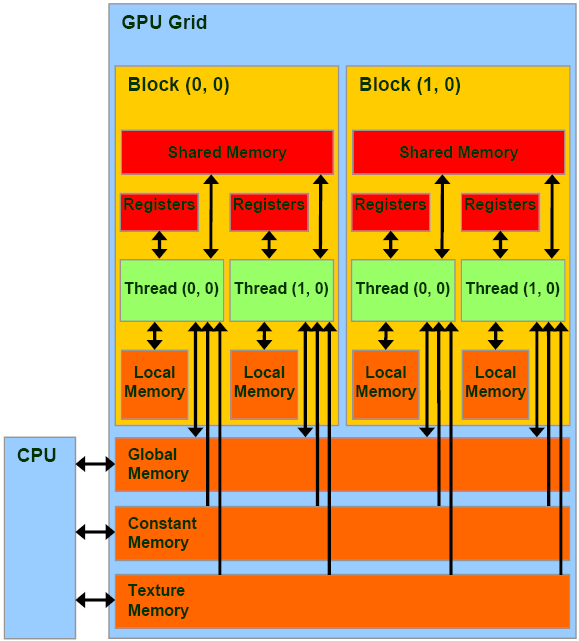
\includegraphics[width=\textwidth]{imgs/cudaMem}
  \caption{The CUDA Memory Model}
  \label{fig:cudaMem}
\end{figure}

The difference between the shared and global memory is the speed. The
shared memory is much faster, but also much smaller (typically 16
KB). Its also inaccessible from threads in different blocks.

This make it challenging to utilise the whole GPU, as the algorithms
needs to be rethought.

One way to do this could be letting each thread fetch it's value
($\phi$ in our case) into the shared memory. Then if the threads are
organized in block where neighbouring threads are in the same block,
each thread can fetch the neighbouring pixels from the shared memory.

Such an optimization creates new challenges, as the threads near the
border cannot cross over to the next blocks shared memory. The
solution is to pad the area around the edges of the blocks, so if a
pixel is on the border, its run by both blocks. This makes us run a
few more threads than we have pixels, but it increases the speed as we
can exploit the shared memory.

A more simple type of optimization, is to use texture memory. GPUs
often need fast access to textures, so it have a texture cache
optimized for 2D spatial locality. This means that fetching data from
a texture will make fetching the neighbouring pixels faster.

\section{Implementation}

After a quick time profiling, we found that \texttt{Reinitialize} is
where our program spends most of its time, so this was the first to be
converted into CUDA.

The following is a very naive conversion. The code is almost the same
as the original in section \ref{sec:reinitialize}, and there are no
clever usage of shared memory or other optimizing tricks.

\begin{lstlisting}
#define GetPhi(phi,x,y,w) phi[x+w*(y)]

__global__ void reinit(float *phi,float* phi0, float* phin, 
                       unsigned int width, unsigned int height) {
    uint x = __umul24(blockIdx.x, blockDim.x) + threadIdx.x;
    uint y = __umul24(blockIdx.y, blockDim.y) + threadIdx.y;

    if (x > width || y > height)
        return;
    
    float xy = GetPhi(phi,x,y,width);

    float phiXPlus = 0.0f;
    float phiXMinus = 0.0f;
    float phiYPlus = 0.0f;
    float phiYMinus = 0.0f;        	
    if (x != width-1) phiXPlus  = (GetPhi(phi,x+1, y,width) - xy);
    if (x != 0)       phiXMinus = (xy - GetPhi(phi,x-1, y,width));
    
    if (y !=height-1) phiYPlus  = (GetPhi(phi,x, y+1,width) - xy);
    if (y != 0)       phiYMinus = (xy - GetPhi(phi,x, y-1,width));

    /* GetPhi(phin,x,y,width) = phiYPlus; */
    /* return; */


    float dXSquared = 0;
    float dYSquared = 0;
    float a = GetPhi(phi0,x,y,width);
    if (a > 0) {
        // formula 6.3 page 58
        float _max = max(phiXMinus, 0.0f);
        float _min = min(phiXPlus, 0.0f);
        dXSquared = max(_max*_max, _min*_min);
                    
        _max = max(phiYMinus, 0.0f);
        _min = min(phiYPlus, 0.0f);
        dYSquared = max(_max*_max, _min*_min);
    } else {
        // formula 6.4 page 58
        float _max = max(phiXPlus, 0.0f);
        float _min = min(phiXMinus, 0.0f);
        dXSquared = max(_max*_max, _min*_min);
                    
        _max = max(phiYPlus, 0.0f);
        _min = min(phiYMinus, 0.0f);
        dYSquared = max(_max*_max, _min*_min);        				
    }

    float normSquared = dXSquared + dYSquared;           
    float norm = sqrt(normSquared);

    // Using the S(phi) sign formula 7.6 on page 67
    //float sign = phi(x,y) / sqrt(phi(x,y)*phi(x,y) + normSquared);
    float sign = GetPhi(phi0,x,y,width) / 
        sqrt(GetPhi(phi0,x,y,width)*GetPhi(phi0,x,y,width) + 1);
    float t = 0.3; // A stabil CFL condition
    GetPhi(phin,x,y,width) = GetPhi(phi,x,y,width) - sign*(norm - 1)*t;


}
\end{lstlisting}

Coping the data, and starting the threads are done in the following code:

\begin{lstlisting}
void cu_Reinit(float* data, 
               unsigned int w,
               unsigned int h,
               unsigned int iterations) {
    float* phiData;
    float* phi0Data;
    float* phinData;

    cudaMalloc((void**)&phiData, sizeof(float)*w*h);
    cudaMalloc((void**)&phi0Data, sizeof(float)*w*h);
    cudaMalloc((void**)&phinData, sizeof(float)*w*h);
    cudaMemcpy((void*)phiData,(void*)data, sizeof(float)*w*h,
               cudaMemcpyHostToDevice);
    cudaMemcpy((void*)phi0Data,(void*)data, sizeof(float)*w*h,
               cudaMemcpyHostToDevice);
    cudaMemcpy((void*)phinData,(void*)data, sizeof(float)*w*h,
               cudaMemcpyHostToDevice);


    CHECK_FOR_CUDA_ERROR();

    const dim3 blockSize(32,16,1);
    const dim3 gridSize(w/blockSize.x, h/blockSize.y);

    for (unsigned int i=0;i<iterations;i++) {
        reinit<<<gridSize,blockSize>>>(phiData,phi0Data,phinData,w,h);
        float* tmp = phiData;
        phiData = phinData;
        phinData = tmp;

        cudaThreadSynchronize();
        CHECK_FOR_CUDA_ERROR();
    }

    cudaMemcpy((void*)data,(void*)phiData,
                sizeof(float)*w*h,cudaMemcpyDeviceToHost);
    CHECK_FOR_CUDA_ERROR();
    cudaFree(phiData);
    cudaFree(phi0Data);
    cudaFree(phinData);
}

\end{lstlisting}

\section{Results \& Conclusion}

The results in table \ref{tbl:cudaRes} are taken from a system with a
1.8 Ghz Intel Core 2 Duo CPU, 4 GB RAM and a 512MB nVidia GeForce
9600M GT. The time is an average of about 100 iterations of the
algorithm.

\begin{table}[h]
  \centering
  \begin{tabular}{|l|r|r|r|}
    \hline    Algorithm & CPU ($\mu s$) & GPU ($\mu s$) & Speedup ($\times$) \\
    % BEGIN RECEIVE ORGTBL numbers
\hline
Reinitialization & 417825 & 136675 & 3.0570697 \\
- with textures & - & 100006 & 4.1779993 \\
\hline
    % END RECEIVE ORGTBL numbers
  \end{tabular}
  \caption{GPU vs. CPU comparison}
  \label{tbl:cudaRes}
\end{table}

% grep Reinit run1.log | grep CUDA | awk '{sum+=$7} END {print "avg=",sum/NR}'

\begin{comment}
#+ORGTBL: SEND numbers orgtbl-to-latex :splice t :skip 2
|------------------+--------+--------+-----------|
|                  | CPU    |    GPU |   Speedup |
|------------------+--------+--------+-----------|
| Reinitialization | 417825 | 136675 | 3.0570697 |
| - with textures  | -      | 100006 | 4.1779993 |
|------------------+--------+--------+-----------|
#+TBLFM: @2$4=@2$2 / @2$3::@3$4=@2$2 / @3$3
\end{comment}

The results shows a significant speedup. Using a quite naive
implementation the speedup is easily tripled on a inexpensive consumer
graphics card.

Using textures to cache lookup, we gain even more performance, going
from 3x to 4x. If we'd had more time more optimization techniques
could have been applied. E.g. using shared memory which most likely
would have improved performance even more.

A visual ilustration of the sppedup can be seen in figure
\ref{fig:cudaComp}. Here the AU logo is morphed into a circle, and
after 30 seconds the GPU version is way ahead of the CPU version.

\begin{figure}[h]
  \centering
  \subfloat[Original AU logo]{
    
\includegraphics[width=0.25\textwidth]{imgs/au-logo}}
  \subfloat[Circle]{
    
\includegraphics[width=0.25\textwidth]{imgs/circle}}    
  \subfloat[GPU version]{
    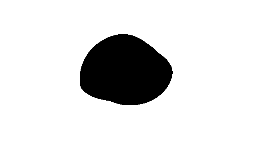
\includegraphics[width=0.25\textwidth]{imgs/auMorphCuda}}
  \subfloat[CPU version]{
    
\includegraphics[width=0.25\textwidth]{imgs/auMorphCpu}}
  \caption{Comparision of CPU vs. GPU on morph}
  \label{fig:cudaComp}
\end{figure}



%%% Local Variables: 
%%% mode: latex
%%% mode: auto-fill
%%% mode: orgtbl
%%% TeX-PDF-mode: t
%%% TeX-master: "../master.tex"
%%% End: 
